%%%%%%%%%%%%%%%%%%%%%%%%%%%%%%%%%%%%%%%%%%%%%%%%%%%%%%%%%%%%%%%%%%% 
%%%%%%%%%%%%%%%%%%%%%%%%%%%%%%%%%%%%%%%%%%%%%%%%%%%%%%%%%%%%%%%%%%% 
%%%%%%%%%%%%%%%%%%%%%%%%%%%%%%%%%%%%%%%%%%%%%%%%%%%%%%%%%%%%%%%%%%% 
\begin{frame}
  \frametitle{Future of accelerator programming}

  \begin{itemize}
  \item \textcolor{red}{\textbf{passive libraries:}} a collection of subroutines
  \item \textcolor{blue}{\textbf{active libraires:}} take an active role in compilation (specialize algorithms, tune themselves for target architecture).
  \end{itemize}

  \begin{center}
    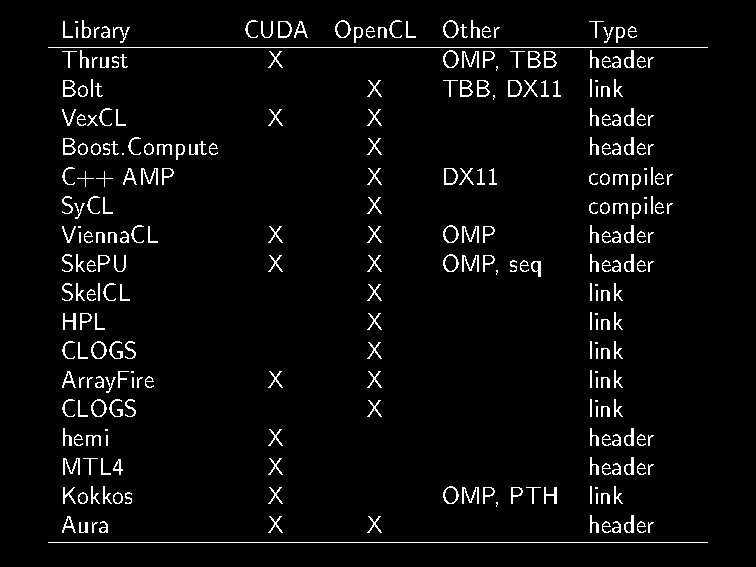
\includegraphics[width=6cm]{images/acc_prog_cpp.pdf}
  \end{center}
  
  reference: \myhref{http://www.soa-world.de/echelon/wp-content/uploads/2014/05/CppNow2014_Future_of_Accelerator_Programming.pdf}{The Future of
    Accelerator Programming in C++, S. Schaetz, May 2014}
  
\end{frame}

%%%%%%%%%%%%%%%%%%%%%%%%%%%%%%%%%%%%%%%%%%%%%%%%%%%%%%%%%%%%%%%%%%% 
%%%%%%%%%%%%%%%%%%%%%%%%%%%%%%%%%%%%%%%%%%%%%%%%%%%%%%%%%%%%%%%%%%% 
%%%%%%%%%%%%%%%%%%%%%%%%%%%%%%%%%%%%%%%%%%%%%%%%%%%%%%%%%%%%%%%%%%% 
% \begin{frame}
%   \frametitle{Future of accelerator programming}

%   \begin{itemize}
%   \item \textbf{Coordination:}
%     \begin{itemize}
%     \item concurrency: asynchronicity, data dependency graph
%     \item memory management (explicit ? implicit ?) / memory layout (SoA, AoS, unordered map, Morton-index, ...)
%     \end{itemize}
    
%   \item \textbf{Computation:}
%     \begin{itemize}
%     \item parallel primitives
%     \item custom accelerator functions
%     \item numerical analysis
%     \item performance portability
%     \item kernel-space exploration / tuning
%     \end{itemize}
%   \end{itemize}

%   reference: \myhref{http://www.soa-world.de/echelon/wp-content/uploads/2014/05/CppNow2014_Future_of_Accelerator_Programming.pdf}{The Future of
%     Accelerator Programming in C++, S. Schaetz, May 2014}
  
% \end{frame}

%%%%%%%%%%%%%%%%%%%%%%%%%%%%%%%%%%%%%%%%%%%%%%%%%%%%%%%%%%%%%%%%%%% 
%%%%%%%%%%%%%%%%%%%%%%%%%%%%%%%%%%%%%%%%%%%%%%%%%%%%%%%%%%%%%%%%%%% 
%%%%%%%%%%%%%%%%%%%%%%%%%%%%%%%%%%%%%%%%%%%%%%%%%%%%%%%%%%%%%%%%%%% 
\begin{frame}
  \frametitle{Complex memory layout for performance}

  \begin{itemize}
  \item How to improve \textcolor{red}{\textbf{space (memory) locality}} in algorithm implementations ?
  \item \textbf{\textit{High Performance Parallelism Pearls}}, \textcolor{darkgreen}{\textbf{Morton order to improve memory locality}}, by Kerry Evans (INTEL), chap. 28
  \item \textbf{matrix transpose}, \textbf{dense matrix multiplication} on Xeon, KNC
  \item Same feature used in some Adaptive Mesh Refinement PDE solver.
  \end{itemize}

  
  \begin{center}
    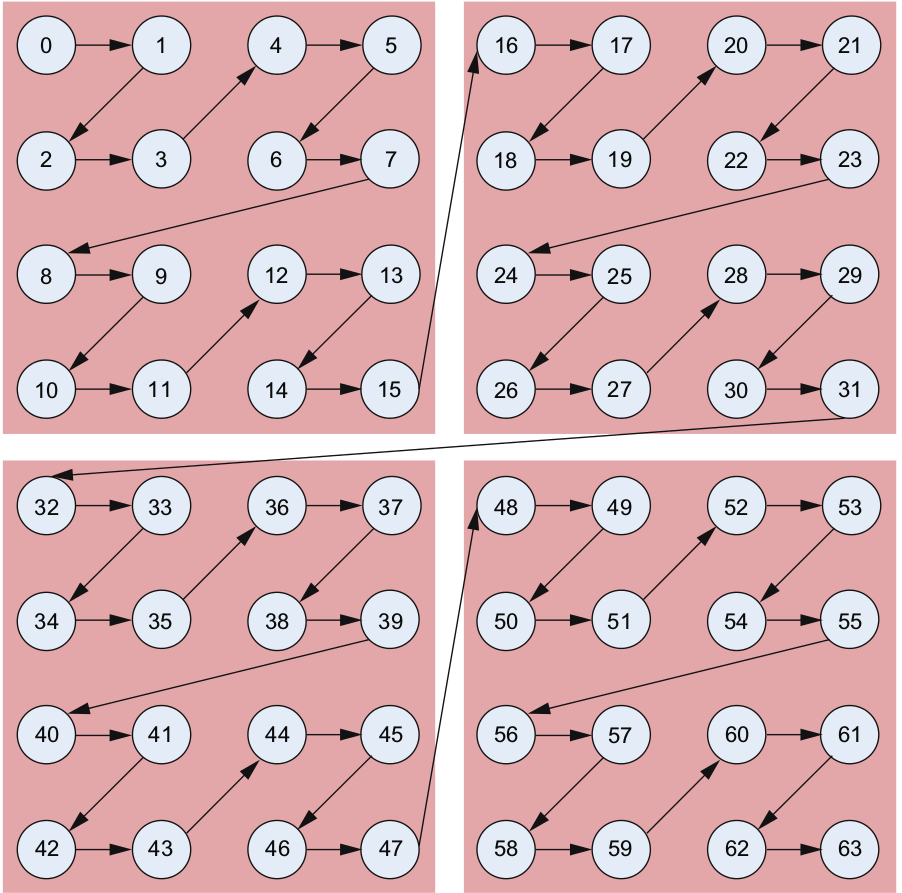
\includegraphics[width=3.5cm]{images/c28_morton_order}
    \hfill
    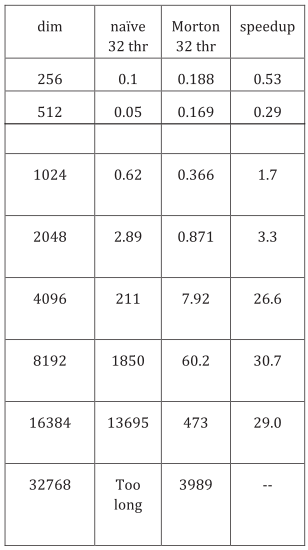
\includegraphics[height=3.5cm]{images/c28_MatrixMult_xeon1}
    \hfill
    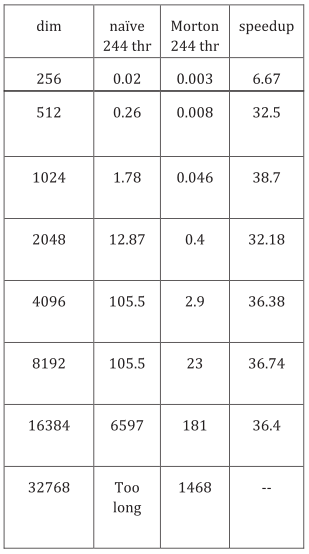
\includegraphics[height=3.5cm]{images/c28_MatrixMult_MIC}
  \end{center}

\end{frame}
